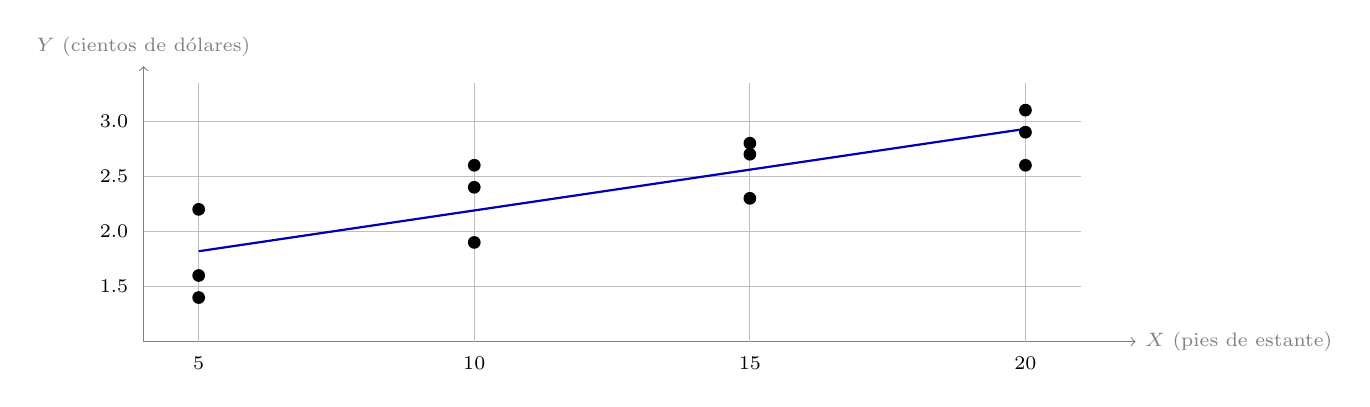
\begin{tikzpicture}[x=0.70cm,y=1.4cm,font=\scriptsize]
    \draw[->,gray] (4,1.0) -- (22,1.0) node[right] {$X$ (pies de estante)};
    \draw[->,gray] (4,1.0) -- (4,3.5) node[above] {$Y$ (cientos de dólares)};
    \foreach \x in {5,10,15,20} {
        \draw[gray!50] (\x,1.0) -- (\x,3.35);
        \node[below=2pt] at (\x,1.0) {\x};
    }
    \foreach \y in {1.5,2.0,2.5,3.0} {
        \draw[gray!50] (4,\y) -- (21,\y);
        \node[left=2pt] at (4,\y) {\y};
    }
    \draw[blue!70!black,thick] plot coordinates {(5,1.82) (20,2.93)};
    \foreach \x/\y in {5/1.6,5/2.2,5/1.4,10/1.9,10/2.4,10/2.6,15/2.3,15/2.7,15/2.8,20/2.6,20/2.9,20/3.1} {
        \fill[black] (\x,\y) circle (2.3pt);
    }
\end{tikzpicture}